\chapter{INTRODUCTION}
\section{Overview}
\vspace{20pt}
Text classification is a construction problem of models which can classify new documents into pre-defined classes. It involves assigning documents into their predefined categories based on their contents. In many real-world scenarios, the ability to automatically classify documents into a fixed set of categories is highly desirable. This allows users to find desired information faster by searching only the relevant categories and not the entire information space. The importance of text classification is even more apparent when the information space is huge such as the World Wide Web \cite{ajose2020performance}.\\
Word embedding is a way to represent a word with fixed-length vector of continuous real numbers. It maps a word in a vocabulary to a latent vector space where words with similar context are in proximity. Through word embedding, a word is converted to a vector that summaries both the word’s syntactic and semantic information. Consequently, word embedding is particularly suitable to be used as feature representations in neural network model for downstream natural language processing task, such as text classification, machine translation, sequence learning \cite{bhoir2017comparative}.\\
\begin{figure}
  \centering 
  \vspace{20pt}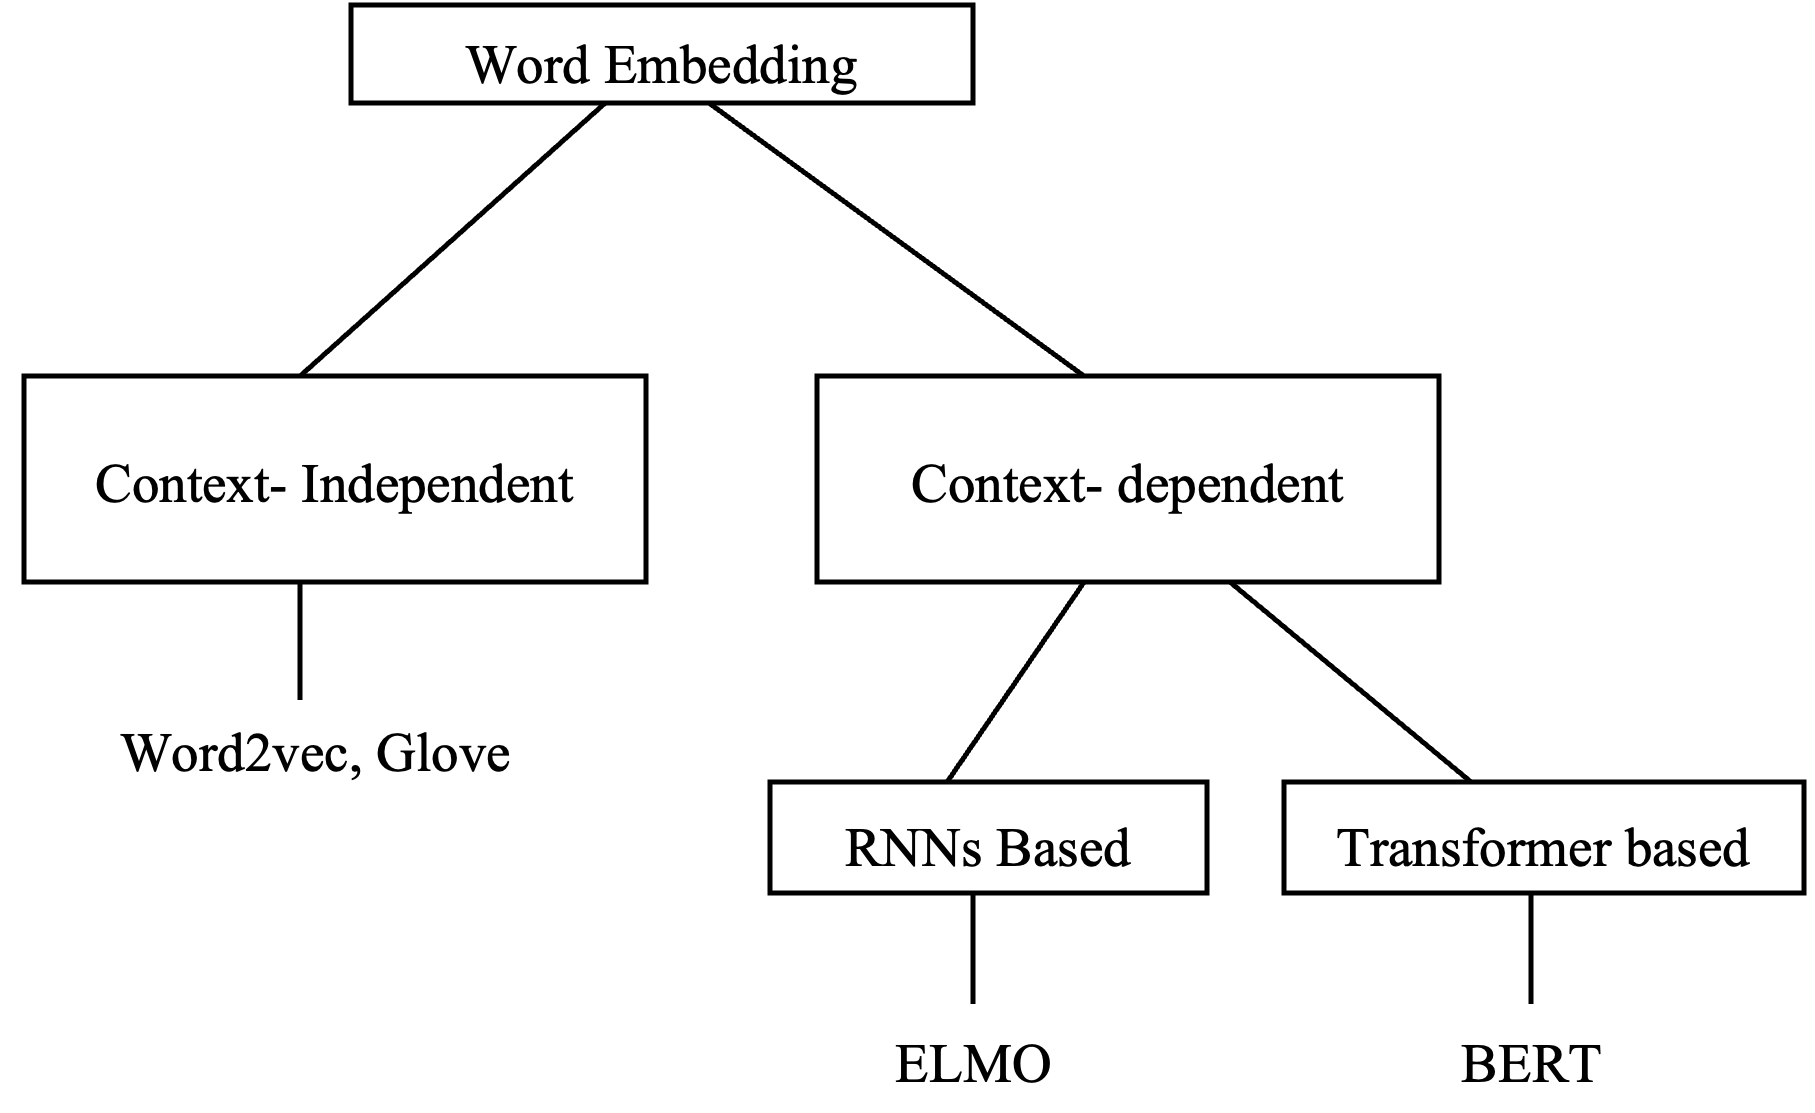
\includegraphics[width=10cm]{images/intro.png}\\
  \caption{A taxonomy of word embedding} 
  \label{fig:taxonomy}
\end{figure}
Finding such representation for words and sentences has been one hot topic over the last few years in the field of Natural Language Processing and has led to many improvements in core NLP task.
This seminar report seeks to compare the effect of different word representation for the Nepali text classification. Here, Word2vec and ELMO word embedding techniques are used for the analysis purpose these are the two category of word representation technique namely context dependent and context independent show in the figure \ref{fig:taxonomy}. All in all, this transformation has two important beneficial properties that is dimensionality reduction for efficient representation and contextual similarity for expressive representations.\\
The remaining part of this seminar report is organized as follow. Literature reviews to this study are described in Chapter 2. In Chapter 3, have described the proposed methodology. The implementation part is described in Chapter 4. Finally, result and conclusion is included in the chapter 5 and 6 respectively.
\subsection{Problem Statement}
The huge unstructured data in the digital world is one of the reasons where the application of various machine learning techniques is possible. However, the complex morphology of text due to various forms of existing consonants and vowel letters make it difficult in feature extraction from the document. Since the different languages are morphologically rich and complex, natural language processing task such as classification and machine translation has become complex because of inappropriate word embedding techniques.
\section{Objective}
\begin{itemize}

  \item {To implement and analysis context dependent and independent word embedding model.}

  \item {To implement SVM and Random Forest Machine learning algorithms for text classification.}

\end{itemize}
\clearpage